\section{Experimental Setup}
\label{sec:setup}

\begin{figure}[H]
\centering
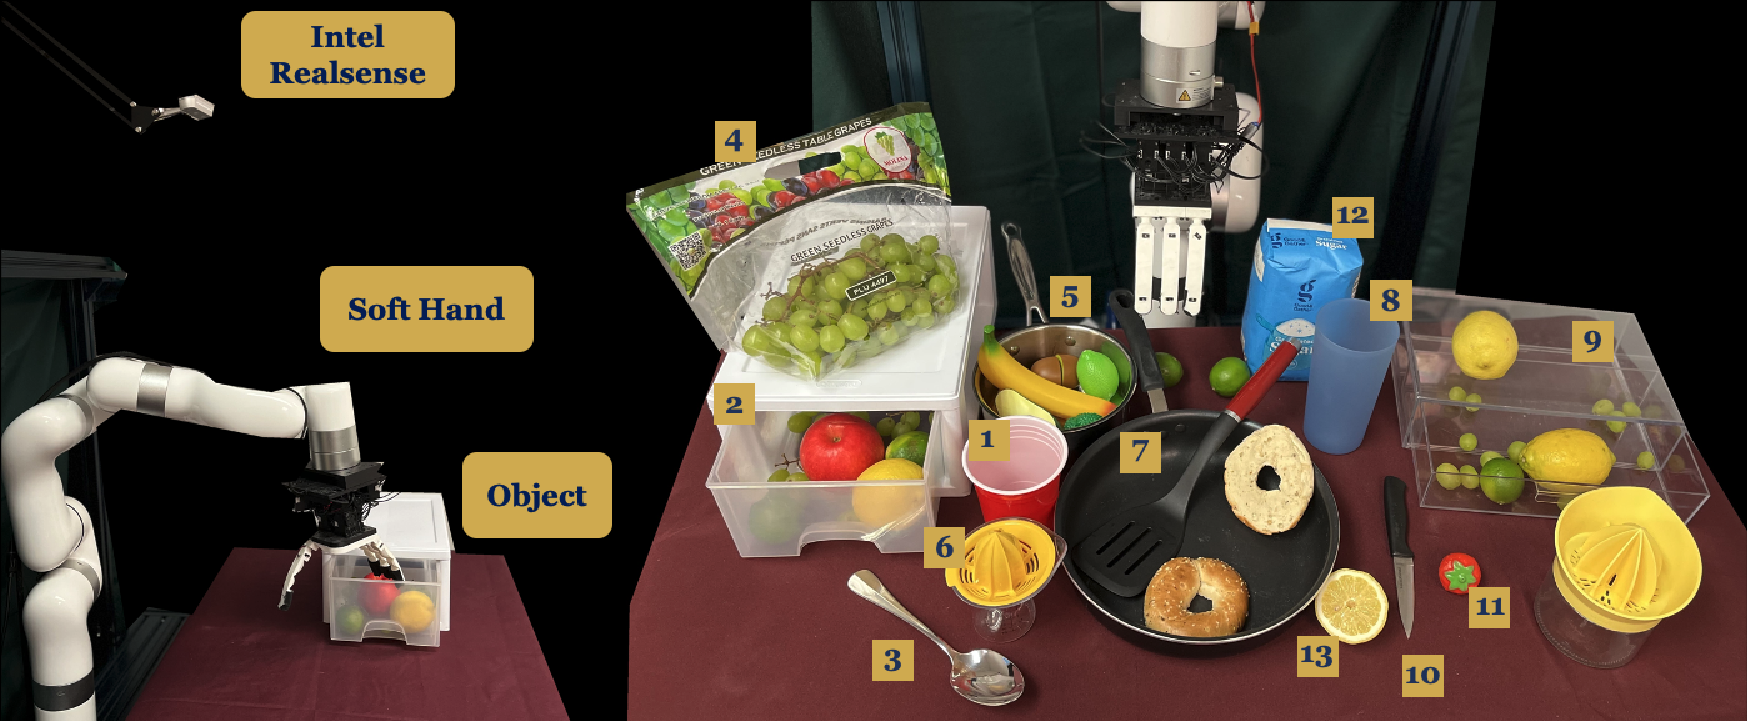
\includegraphics[width=\linewidth]{figs/workspace.pdf}
\vspace{-0.2in}
  \caption{\small \textbf{Left}: Workspace Setup. We place an Intel RealSense camera above the robot to maintain an egocentric viewpoint, consistent with the affordance model's training data. \textbf{Right}: Thirteen objects used in our experiments.}
 \label{fig:workspace}
 \vspace{-0.15in}
\end{figure}

\subsection{Task Setup} We introduce 9 tabletop tasks: \textit{Pick Cup}, \textit{Pour Cup}, \textit{Open Drawer}, \textit{Pick Spoon}, \textit{Scoop Grape}, \textit{Stir Spoon}, \textit{Pick Grape}, \textit{Flip Bagel}, and \textit{Squeeze Lemon}. For all tasks, we randomize the position of the object on the table, as well as use train and test objects with different shapes and appearances to test for generalization. See Figure~\ref{fig:workspace} for a depiction of the robot's workspace and the objects we use in our experiments.

We define the success criteria in each of our 9 tasks as follows:

\begin{itemize}
    \item Pick Cup: Cup must leave table surface and stay grasped throughout trial.
    \item Pour Cup: Cup must be grasped throughout trial and also rotate so that the top of the cup is at a lower height than the base.
    \item Open Drawer: Drawer is initially slightly open so that it can be grasped. By the end of the rollout, the drawer should be at least 1 centimeter more open than it was at the beginning.
    \item Pick Spoon: The spoon must not be in contact with the table at the end of the trial.
    \item Stir Spoon: The spoon base must rotate around the jar/pot at least 180 degrees while grasped.
    \item Scoop Grape: The spoon must have a grape at the end of the trial while being held by the soft hand.
    \item Pick Grape: All grapes must be held by the hand above the table surface. In particular, if any single grape falls due to a weak stem, this is considered a failure.
    \item Flip Bagel: The side of the bagel that is facing up at the end of the trial should be opposite the side facing up at the beginning.
    \item Squeeze Lemon: The lemon should be grasped securely on top of the juicer.
\end{itemize}

\subsection{Online Fine-Tuning Setup}

To achieve real-world learning with the soft robot hand, we pretrain an internet affordance model as a prior for robot behavior.  As explained in Section \ref{sec:method}, we train one language-conditioned model on all data.  At test time, we use this as initialization for our real-world fine-tuning. The fine-tuning is done purely in the real world.  An operator runs 10 warmup episodes of CEM, followed by 20 episodes that continually update the noise distribution, improving the policy. We train a residual VAE policy that trains on the top ten CEM rollouts to predict the noise given the image and affordance outputs. Over all our experiments, we collect data for several thousands of rollouts for over \textbf{100 hours} of real world data collection.

\subsection{Datasets and Affordance Model Parameters}

We use data from Ego4D \cite{ego4d}, EpicKitchens-100 \cite{EPICKITCHENS}, and HOI4D \cite{hoi4d}.  After filtering for clips of sufficient length, clips that involve grasping objects with the right hand, and clips that have language annotations, we used 64666 clips from Ego4D, 9144 clips from EpicKitchens, and 2707 clips from HOI4D. In total, we use a dataset of 76517 samples for training our model.

For our contact location model, we use the visual encoder from \cite{r3m} to encode the image as a 512-dimensional vector. We use the spatial features of the encoder to upsample the latent before applying a spatial softmax to return the contact heatmap. This consists of three deconvolutional layers with 512, 256, and 64 channels in that order.

To predict wrist rotation and grasp pose, we use the language encoder from \cite{Clip} to compress the language instruction to a 512-dimensional vector. We concatenate the visual and language latents and pass it through a transformer with eight heads and six self-attention layers. We pass the result of the transformer through an MLP with hidden size 576, and predict a vector of size 48: the first 3 dimensions are the axis-angle rotations; the last 45 dimensions are the joint angles of the hand. These correspond to the parameters output by Frankmocap \cite{FrankMocap_2021_ICCV}, which we used to get ground truth hand pose in all the datasets.

We jointly optimize the L2 loss of the contact location $\mu$, the wrist rotation $\theta_\text{wrist}$ and grasp pose $P$. The weights we used for the losses are $\lambda_\mu = 1.0, \lambda_\theta = 0.1, \lambda_P = 0.1$. We train for 70 epochs with an initial learning rate of 0.0002, and a batch size of 224. We used the Adam optimizer \cite{kingma2014adam} with cosine learning rate scheduler. We trained on a single NVIDIA RTX A6000 with 48GB RAM.

\subsection{Hardware Setup}

We use a 6-DOF UFactory xArm6 robot arm for all our experiments. We attach it to a 16-DOF Soft Hand using a custom, 3D-printed base. We use a single, egocentric RGBD camera in order to capture the 3D location of the object in the camera frame. We calibrate the camera so that the predictions of the affordance model can be converted to and executed in the robot frame. The flexibility of the robot hand also makes it robust to collisions with objects or unexpected contact with the environment. 

\subsection{Safety} 

In our fine-tuning experiments, there is a particular focus on the safety of the robot system and the environment. The soft hand allows the policy to perform high-contact manipulation tasks without breaking because of its compliance. Our method takes advantage of the compliance as it performs thousands of iterations in the real world.

While the end-effector is soft, the arm is not. Because it is susceptible to damage when colliding with the environment, we constrain the arm's velocity and ensure that the arm stays above the tabletop. The rollout will be terminated if the arm's dynamics controller senses that the arm collided aggressively with the environment.
 